\documentclass{beamer}
\usepackage{graphicx}
\graphicspath{ {./images/} }
\usetheme{metropolis}

\begin{document}

\title{Analyse de couverture urbaine par homologie persistante : cas du 
    développement des transports publics}
\author{Harnisch Elowan ; 14002}
\date{\today}

\maketitle

\begin{frame}
    \frametitle{Homologie persistante}
    L'homologie persistante est une méthode pour calculer des caractéristiques
    topologiques d'un espace. En l'occurrence ici pour déterminer des "trous" dans
    une couverture par les transports publics
    
\end{frame}

\begin{frame}
    \frametitle{Définitions}
    \begin{block}{Simplexe}
        Généralisation d'un triangle en dimension $n$
    \end{block}

    \begin{block}{Complexe simplicial}
        Un ensemble de simplexes de dimension non forcément égales
    \end{block}

    \begin{block}{Filtration}
        Suite croissante pour l'inclusion de complexes simplicials
    \end{block}

    \begin{figure}
        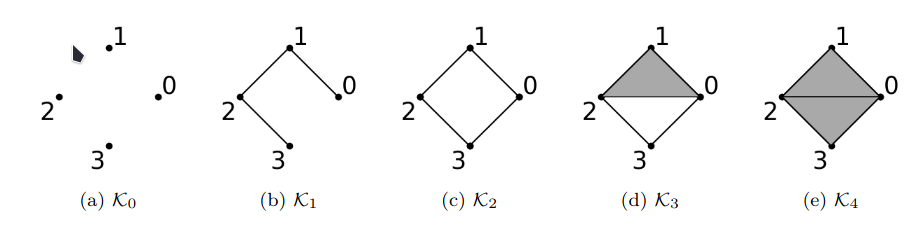
\includegraphics[width=\textwidth]{filtration}
        \centering
        \caption{Exemple de filtration}
    \end{figure}
    
\end{frame}

\begin{frame}
    \frametitle{Méthode}
    \itemize{
        \item Construction d'une filtration de complexes simplicials via 
            les complexes pondérés de Vietoris-Rips
        \item Construction de la matrice de bordure
        \item Réduction de cette matrice par l'algorithme standard
        \item Construction du diagramme de persistance
    }
    \begin{figure}
        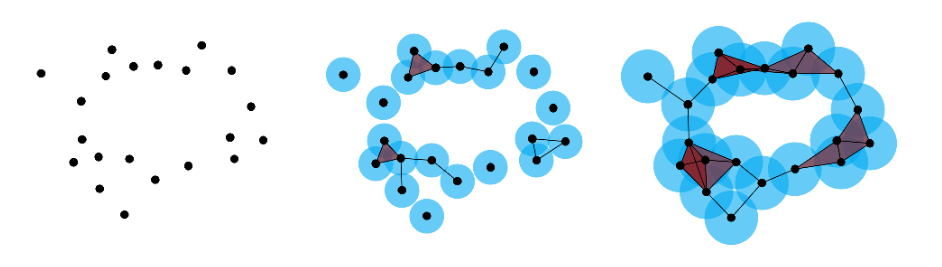
\includegraphics[width=0.7\textwidth]{cech}
        \centering
        \caption{Construction de Vietoris-Rips}
    \end{figure}
    
\end{frame}

\begin{frame}
    \frametitle{Illustration}
    \begin{figure}
        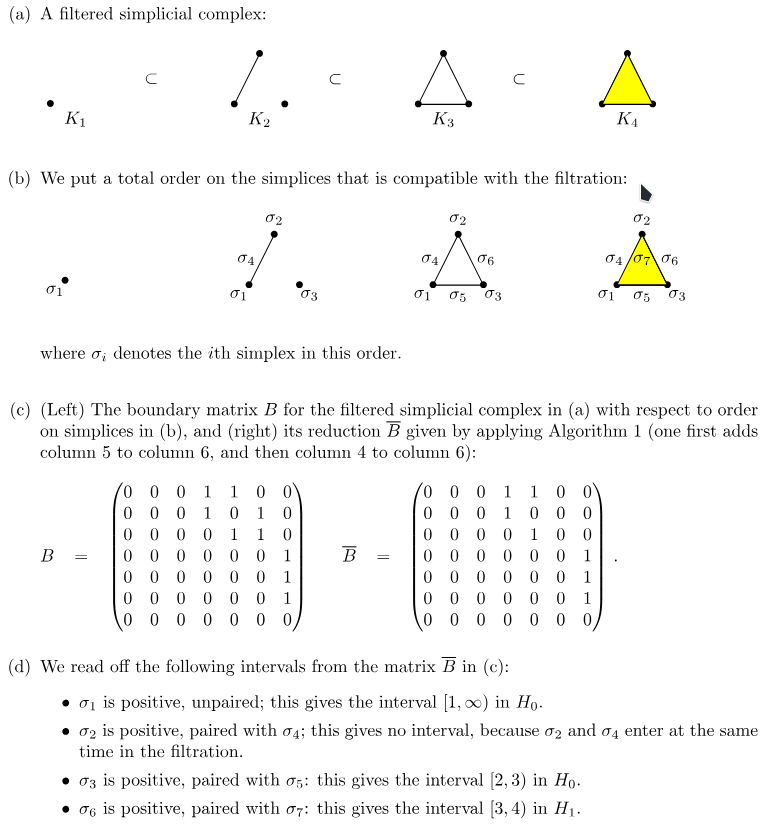
\includegraphics[width=0.7\textwidth]{pipeline}
        \centering
        \caption{Pipeline de la méthode}
    \end{figure}

\end{frame}

\begin{frame}
    \frametitle{Définition des distances}
    
    \begin{block}{Distance}
        On définit la distance $d$ entre deux stations de metro $x$ et $y$ : 
        $$ d(x,y) =  min(t_{pied}(x,y), t_{voiture}(x,y))$$
    \end{block}
\end{frame}

\begin{frame}
    \frametitle{Récupération des données}
    Pour le calcul des temps de trajet :  apidocs.geoapify.com

    Pour la récupération des stations et des temps d'attentes moyens : transport.data.gouv.fr
\end{frame}

\begin{frame}
    \frametitle{Résultats so far so good}
    Pour marseille 
    \begin{figure}
        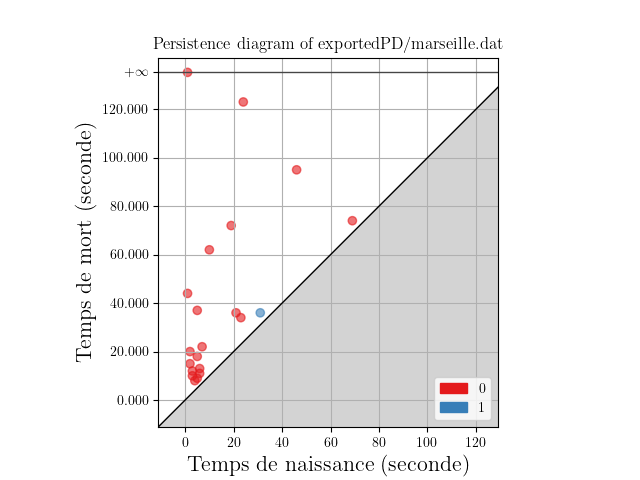
\includegraphics[width=0.7\textwidth]{pd_marseille}
        \centering
        \caption{Diagramme de persistance}
    \end{figure}
\end{frame}

\begin{frame}
    \frametitle{Conclusion}
    Restant :
    \itemize{
        \item Compréhension des résultats précédents + correction du programme
        si necéssaire
        \item PreTraitement des informations sur Paris/Toulouse/Rennes 
        \item Conclure
    }
    
\end{frame}

\end{document}